\chapter{Testy Oprogramowania}
\label{cha:testy}

Rozdział ten jest poświęcony krótkiemu opisowi testów, którym poddano oprogramowanie w celu sprawdzenia poprawoności działania.
Skupiają się one głównie na poprawności tworzenia struktur AGDS oraz przytaczają wybrane dane dotyczące szybkości tworzenia tych struktur.

\section{Testy poprawności tworzenia struktur AGDS}
\label{sec:testAgds}

Podstawowe test działania oprogramowania opierają się na przykładach zamieszczonych w \cite[s. 228 - 232]{Horzyk}. Przedstawiono tam
kompletny przykład tworzenia struktury AGDS i jej końcowy wygląd. Jeden z przykładów włączony został do zbioru testów automatycznych, zapewniając
w ten sposób częste sprawdzanie najważniejszej funkcjonalności i umożliwiając szybkie wykrywanie błędów.

Test polega na zbudowaniu struktury AGDS modelującej przykładowe sekwencję. Sam proces budowy AGDS, jak i finalny wygląd sieci można znaleźć
w \cite[s.232]{Horzyk}. 

Struktura tworzona jest na podstawie 5 sekwencji uczących, wg wzoru przedstawionego w rozdziale~\ref{cha:budowaGrafu}. 

Sekwencje testowe: $S_1 = \{e1, e2, e3\}, S_2=\{e4, e5, e2, e6\}, S_3 = \{e7, e5, e2, e8\}, S_4 = \{e7, e9, e8\}, S_5=\{e4, e2, e3\}$.

Tabela \ref{tab:test} przedstawia konfrontację wynikowych wag krawędzi AGDS przedstawionych w \cite[s. 232]{Horzyk} i obliczonych przez program.
Widać, iż niewielkie różnice wynikają z dokładności obliczeń numerycznych i nie są związane z niepoprawnością działania implementacji.
\begin{table}[!h]
\centering
\caption{Wyniki tworzenia struktury AGDS dla sekwencji testowych}
\label{tab:test}
\begin{tabular}{ccc}
\hline
Krawędzie  & Waga teoretyczna & Waga wyliczona przez aplikację\\
\hline
\multicolumn{3}{c}{Każda sekwencja jednokrotnie}\\
\hline
$e1 \leadsto e2$ & 1.0  & 1.0\\
$e1 \leadsto e3$ & 0.66  & 0.6666\\
$e2 \leadsto e3$ & 0.66  & 0.6666\\
$e2 \leadsto e6$ & 0.4  & 0.4\\
$e2 \leadsto e8$ & 0.4  & 0.4\\
$e4 \leadsto e2$ & 0.86  & 0.85714\\
$e4 \leadsto e3$ & 0.4  & 0.4\\
$e4 \leadsto e5$ & 0.66  & 0.6666\\
$e4 \leadsto e6$ & 0.29  & 0.2857\\
$e5 \leadsto e2$ & 1.0  & 1.0\\
$e5 \leadsto e6$ & 0.4  & 0.4\\
$e5 \leadsto e8$ & 0.4  & 0.4\\
$e7 \leadsto e2$ & 0.4  & 0.4\\ 
$e7 \leadsto e5$ & 0.66  & 0.6666\\
$e7 \leadsto e8$ & 0.59  & 0.5882\\
$e7 \leadsto e9$ & 0.66  & 0.6666\\
$e9 \leadsto e8$ & 1.0  & 1.0\\
\hline
\multicolumn{3}{c}{$S_1, 5 S_2, S_3, 3 S_4, 2 S_5$}\\
\hline
$e1 \leadsto e2$ & 1.0  & 1.0\\
$e1 \leadsto e3$ & 0.66  & 0.6666\\
$e2 \leadsto e3$ & 0.5  & 0.5\\
$e2 \leadsto e6$ & 0.71  & 0.7142\\
$e2 \leadsto e8$ & 0.2  & 0.4\\
$e4 \leadsto e2$ & 0.78  & 0.7826\\
$e4 \leadsto e3$ & 0.25  & 0.25\\
$e4 \leadsto e5$ & 0.83 & 0.8333\\
$e4 \leadsto e6$ & 0.38  & 0.3846\\
$e5 \leadsto e2$ & 1.0  & 1.0\\
$e5 \leadsto e6$ & 0.53 & 0.5882\\
$e5 \leadsto e8$ & 0.15  & 0.1538\\
$e7 \leadsto e2$ & 0.22  & 0.2222\\ 
$e7 \leadsto e5$ & 0.4  & 0.4\\
$e7 \leadsto e8$ & 0.63  & 0.6285\\
$e7 \leadsto e9$ & 0.86  & 0.8571\\
$e9 \leadsto e8$ & 1.0  & 1.0\\
\end{tabular}
\end{table}


\section{Inne testy i spostrzeżenia}
\label{sec:inneTesty}

Tabela \ref{tab:kontekstTest} ilustruje czas rozbudowy grafu AGDS, w zaeżności od przyjętej długości kontekstu.  Za każdym razem
struktura AGDS budowana była od początku, z wykorzystaniem tej samej sekwencji uczącej, zmieniała się jedynie wartość pola konfiguracyjnego
\texttt{max\_sentence\_length} (kolejno 4, 8 i 12).

\begin{table}[!h]
\centering
\caption{Czas tworzenia grafu AGDS w zależności od wielkości kontekstu}
\label{tab:kontekstTest}
\begin{tabular}{ccc}
\hline
Początkowa ilość węzłów  & Początkowa ilość krawędzi & Czas wstawiania pojedynczej strony[s]\\
\hline
\multicolumn{3}{c}{Maksymalna długość kontekstu 4}\\
\hline
0 & 0 & 3.916 \\
242 & 566 & 18.659 \\
1681 & 8494 & 11.610 \\
1705 & 8573 & 13.768 \\
1915 & 9577 & 16.308 \\
\hline
\multicolumn{3}{c}{Maksymalna długość kontekstu 8}\\
\hline
0 & 0 & 5.57\\
242 & 1246 & 20.464\\
1681 & 12 622 & 24.323\\
1705 & 23 065 & 20.608 \\
1915 & 29 167 & 34.566 \\
\hline
\multicolumn{3}{c}{Maksymalna długość kontekstu 12}\\
\hline
0 & 0 & 6.43 \\
242 & 1854 & 17.539 \\
1681 & 7493 & 24.698 \\
1705 & 23 309 & 38.437 \\
1915 & 33 137 & 42.324 \\
\hline
\end{tabular}
\end{table}

\begin{figure}[!h]
    \centering
    \label{graph:wplyw_kontekstu}
    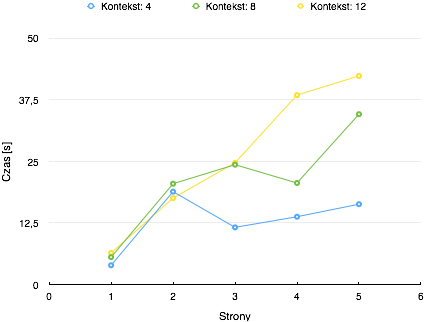
\includegraphics[width=0.8\textwidth]{wplyw_kontekstu}
    \caption{Ilustracja zmiany czasu zapisywania strony w zaleźności od długości kontekstu.}
\end{figure}

\begin{figure}[!h]
    \centering
    \label{graph:wplyw_kontekstu}
    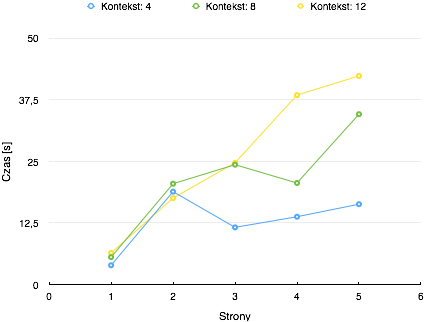
\includegraphics[width=0.8\textwidth]{wplyw_kontekstu}
    \caption{Ilustracja rosnącej liczby krawędzi w zaleźności od długości kontekstu.}
\end{figure}

Jak widać długość kontekstu ma znaczący wpływ na ilość krawędzi grafu, jak i na czas tworzenia struktury. Natomiast ilość węzłów pozostaje bez zmian, co jest zrozumiałe,
ponieważ kontekst określa maksymalną długość połączenia między neuronami, natomiast nie ma wpływu na ich ilość. 

Na rysunku \ref{graph:grafAgds} przedstawiona jest graficzna ilustracja   struktury AGDS zbudowanej na podstawie artykułu znajdującego się pod adresem \url{http://en.wikipedia.org/wiki/Content_(media)}.
Składa się ona z 299 wierzchołków, i 858 krawędzi, kolor i wielkość wierzchołka odpowiadają częstotliowści występowania(i większy, tym częściej występuje. Wierzchołki o tym samym
kolorze występują tą samą liczbę razy). Można zauważyć, iż w tekście znajduje się kilka słów, występujących często i posiadających wiele połączeń. Z analizy grafu dokonanej z poziomu
aplikacji wynika, iż są to w większości słowa z listy \emph{stopwords}, takie jak \emph{the}, \emph{an}, czy \emph{of}(artykuł pisany jest w języku angielskim). Jednak figuruje wśród nich 
również słowo \emph{content}, znajdujące się w tytule artykułu.
Ciekawm zjawiskiem są podgrafy niepołączone z główną strukturą. Przedstawiają one prawdopodobnie definicje uzywające fachowego języka, który nie pojawia się w innych częściach artykułu.

\begin{figure}[!h]
    \centering
    \label{graph:grafAgds}
    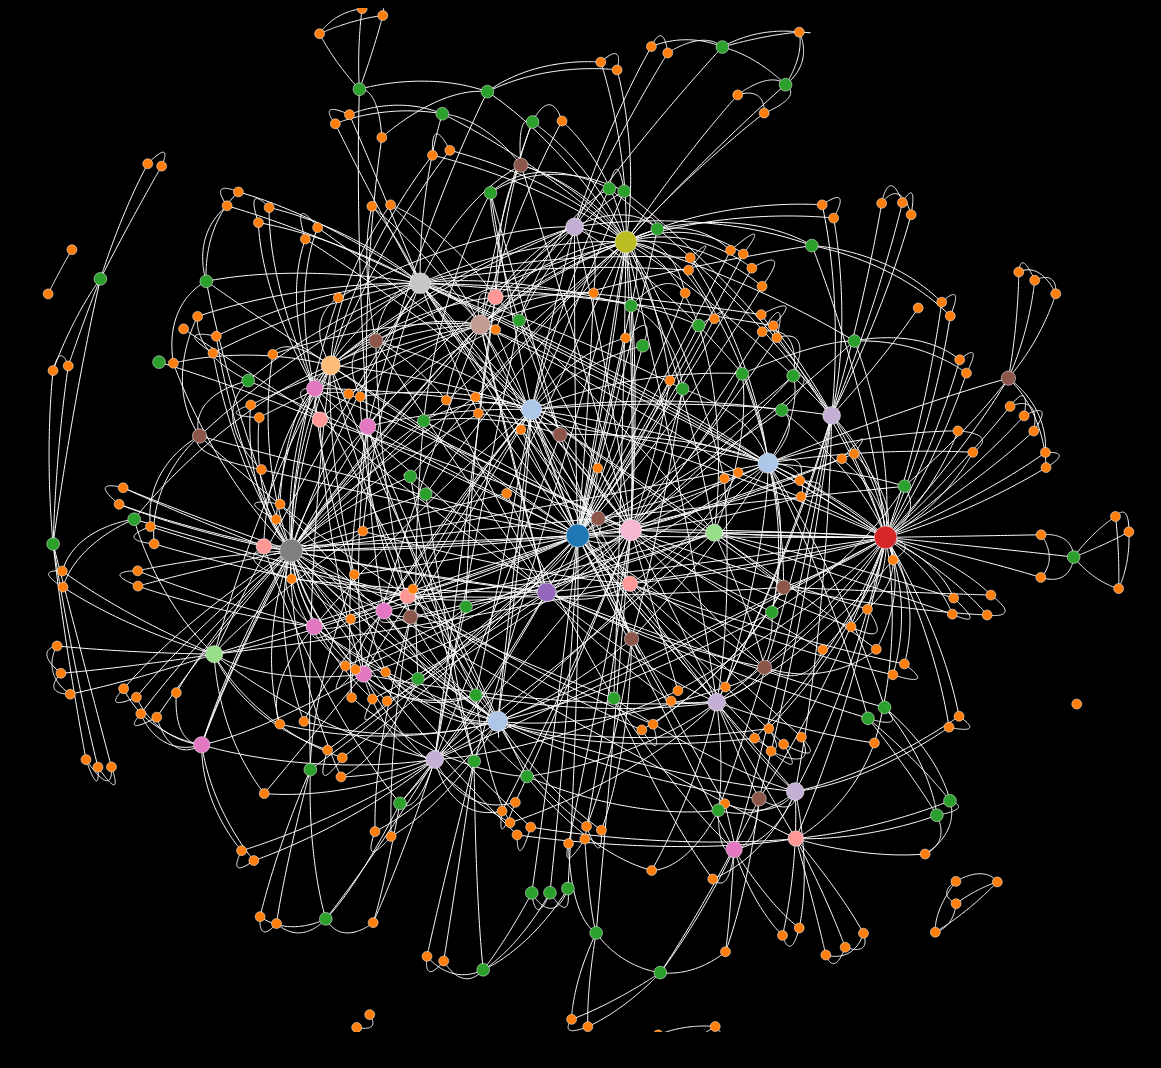
\includegraphics[width=\textwidth]{anakg}
    \caption{Graficzna ilustracja grafu AGDS.}
\end{figure}
